\chapter{Metodologia} \label{cap3}
Os métodos de identificação de sistemas não lineares de áudio podem ser divididos em três etapas: excitação do sistema com um sinal controlado, gravar a saída do sistema e por fim descrever o sistema estudado por uma relação entre a saída dado uma determinada entrada. A escolha dos sinais é uma etapa crucial para que se realize uma identificação de qualidade do sistema estudado\cite{novakdissertation}.

\section{Sinais de Excitação}
\subsection*{Ruído Gaussiano Branco (\textit{White Gaussian Noise (WGN)})}
Um WGN é um sinal definido no tempo como um processo aleatório de média igual a zero. Por ser um processo aleatório, não há como definir o ruído temporalmente. É um ruído puramente aleatório com um espectro de frequência plano e que faz do WGN um excelente sinal de teste \cite{novakdissertation}

\subsection*{Sinais Pseudo Aleatórios}
A geração de um WGN por ser um processo aleatório é uma tarefa muito complicada, talvez impossível de ser feita, mas é possível aproximar sequências com amplitudes binárias (geralmente 0 e 1) com funções de auto correlação e densidade de potência espectral muito semelhantes as funções que compõem um WGN. As vantagens de sinais pseudo aleátorios é a reprodução exata da mesma forma de onda, ou seja, pode ser reproduzido exatamente como foi caracterizado por várias vezes, isso permite sincronizar ao longo do tempo, uma média do sinal. Porém para a caracterização de sistemas não lineares é inviável, uma vez que os valores das amplitudes (0 e 1) são invariáveis a séries de potência. Para evitar esse tipo de problema foi proposto por \cite{haber1999nonlinear} sinais pseudo aleatórios com multiplos níveis de amplitudes para a identificação de sistemas não lineares \cite{novakdissertation}.

\subsection*{Sinais Harmônicos puro e multitonal}
É um dos métodos mais simples para identificação, consiste na aplicação de um sinal senoidal de uma única frequência, onde a resposta do sistema é estudada no domínio da frequência para a estimação de parâmetros, como por exemplo a distorção total harmônica.
\begin{equation}
x(t) = A_{0} exp(j (2\pi f t + \phi_{0}))
\end{equation}

A senóide $x(t)$ pura definida na equação acima é constituida por uma amplitude $A_{0}$, uma única frequência $f$ e a fase $\phi_{0}$. Imaginando que se deseja caracterizar um sistema de áudio através da resposta do sistema até o límite da frequência audível, seriam necessário repetir o processo alterando a frequência do sinal por pelo menos $20000$ vezes para capturar todo o espectro audível.
Para realizar um processo com menos iterações, utiliza-se um sinal multitonal composto por vários harmônicos de diferentes frequências (não necessáriamente frequências múltiplas da frequência fundamental). Esse tipo de sinal pode ser descrito de várias formas, uma delas por exemplo é:
\begin{equation}
x(t) = \sum_{k=0}^{N-1}B_{k} exp(j (2\pi k f_{0} t + \phi_{k}))
\end{equation}

Onde $B_{k}$,$kf_{0}$ e $\phi_{,k}$ são respectivamente, a amplitude, frequência e fase da k-ésima contribuição harmônica.

\subsection*{\textit{Swept Sines}} \label{Sweptsines}
\textit{Swept Sines} são sinais senoidais que com o passar do tempo variam a sua frequência instantânea, cobrindo uma faixa do espectro de frequências.
São muito usados na área de comunicação em sonares e radares, mas também podem ser utilizado em sistemas de áudio para cobrir toda a frequência audível.

Um sinal desse tipo que aumenta a sua frequência exponencialmente é definido como:
\begin{equation}
x(t) = sin (2\pi f_{1}L [exp(\dfrac{t}{L})])
\label{sinal exponencial}
\end{equation}

Onde, a frequência instantânea é dada por:
\begin{equation}
f_{i}(t) = f_{1} exp(\dfrac{t}{L})
\end{equation}

o atraso de grupo $t_{f}$ é a função inversa da frequência instantânea $f_{i}$ e é dada por:
\begin{equation}
t_{f}(f) = L \ln(\dfrac{f_{i}}{f_{1}})
\end{equation}

A duração de tempo $T$ do sinal $x(t)$ pode ser expressa em função da frequência $f_{1}$ e da frequência $f_{2}$ que são, respectivamente, a frequência em que o sinal começa e a frequência em que o sinal termina\cite{novak2010nonlinear}.

\begin{equation}
T = L \ln(\dfrac{f_{2}}{f_{1}})
\label{Equação 5.10}
\end{equation}

A imagem abaixo mostra como a frequência do sinal varia com o passar do tempo.
\begin{figure}[!htb]
	\centering
	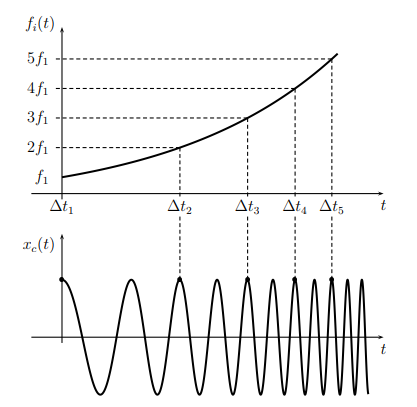
\includegraphics[width=0.6\linewidth]{figuras/SSS}
	\caption{Em cima: Frequência instantânea $f_{i}$. Embaixo: \textit{swept signal} sincronizado. Autor: \cite{novak2010chebyshev}}
	\label{fig:sss}
\end{figure}

\subsection*{Escolha do sinal de excitação}
Para a realização dos testes em um amplificador analógico foi escolhido o \textit{Swept Sine} por que ele tem uma banda de frequências definida, uma melhor resolução em frequência e qualquer ruído que ocorra durante os testes não comprometem a caracterização.

O ruído branco não foi escolhido por que a sua resposta em frequência acaba sobrepondo os efeitos não lineares dos amplificadores que consistem em gerar harmônicos com frequências mais altas e também por que ao aplicar ruído branco é impossível de excitar possíveis modos de ressonância.

\section{Caracterização}
\subsection*{Métodos de caracterização para os modelos de Volterra}
Existem vários métodos que são utilizados para a identificação de sistemas não lineares por séries de volterra, alguns já citados na seção \ref{Volterra}, como o método baseado nos impulsos ponderados de Dirac, realizado por \cite{schetzen1974theory} e as identificações dos \kernels no domínio da frequência, utilizando a GFRF e a NOFRF. Todos esses métodos enfrentam o problema da quantidade de parâmetros necessários para representar sistemas de maiores ordens por séries de Volterra, sendo assim, muito pouco utilizados \cite{novakdissertation}.

\subsection*{Métodos de caracterização para os modelos de Wiener e Hammerstein}
Os métodos de identificação pelos modelos de Wiener e Hammerstein são feitos para modelos paramétricos e não paramétricos. Se o modelo é paramétrico, a função não linear pode ser representada por funções polinomiais ou geralmente por séries ortogonais, assim possuem um número limitado de parâmetros a serem definidos \cite{novakdissertation}. Através de iterações de testes, determina-se as partes lineares e não lineares de um sistema não linear, separadamente. Se o modelo é não paramétrico, a identificação dos modelos de sistemas não lineares é feita através de uma estimação de uma função não linear que serve como uma representação polinomial do sistema \cite{greblicki2004nonlinearity}. 

\subsection*{Método de caracterização baseado na convolução não linear}
Esse método utiliza os sinais de excitação de um sistema não linear descritos na subseção \ref{Sweptsines}. Esses sinais possuem uma frequência instantânea que se modifica exponencialmente com o passar do tempo. O método proposto por Farina em \cite{farina2001non} consiste em excitar o sistema em análise com um \textit{Swept Sine} e gravar a saída do sistema. Em seguida	realiza-se um inversão temporal do sinal de excitação que é utilizado para realizar uma convolução com a resposta gravada do sistema em análise. Após essa convolução, obtém-se uma função constituída por $\delta(t)$, impulsos de Dirac. A saída do sistema não linear em análise consiste no sinal de excitação mais os harmônicos gerados pela saturação do sinal, convoluindo o sinal gravado na saída com o sinal de excitação invertido no tempo gera uma resposta impulsional mostrada na figura \ref{fig:nlcir}.

\begin{figure}[!htb]
	\centering
	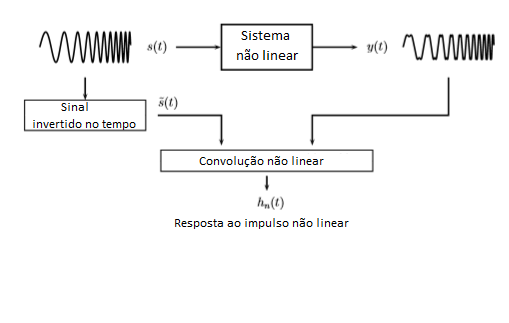
\includegraphics[width=0.9\linewidth]{figuras/NLCM}
	\caption{Diagrama de blocos do método baseado em convolução não linear. Autor: \cite{novakdissertation}}
	\label{fig:nlcm}
\end{figure}

A figura \ref{fig:nlcm} mostra os sinais $s(t)$ e $y(t)$ que são respecticamente, o sinal senoidal que varia exponencialmente na frequência e a saída do sistema em análise. O sinal $\overline{s}(t)$ é o sinal $s(t)$ invertido temporalmente. A convolução entre $y(t)$ e $\overline{s}(t)$ pode ser expressa por:
\begin{equation}
y(t) \ast \overline{s}(t) = \sum_{m=1}^{\infty}h_{m}(t + \Delta t_{m})
\label{kernel}
\end{equation}
Onde, $h_{m}$ é a resposta não linear ao impulso e $\Delta t_{m}$ é a diferença de tempo entre a primeira resposta impulsional e a m-ésima resposta do sistema, onde a primeira resposta define a parte linear do sistema em análise. Dessa forma é possível separar temporalmente cada resposta ao impulso, a partir do valor de $\Delta t_{m}$ como mostra a figura abaixo:

\begin{figure}
	\centering
	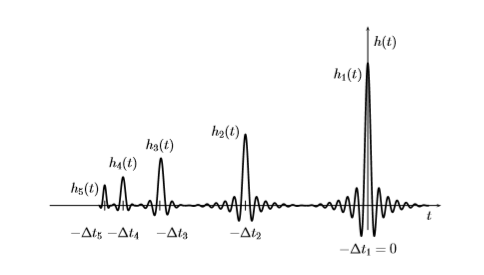
\includegraphics[width=0.6\linewidth]{figuras/NLCIR}
	\caption{Resposta ao impulso do sistema em análise. Autor: \cite{novakdissertation}}
	\label{fig:nlcir}
\end{figure}

Através do uso da Transformada de Fourier de cada resposta ao impulso é obtida a resposta frequêncial de cada impulso como mostra a figura \ref{fig:nlcfr}
\begin{figure}
	\centering
	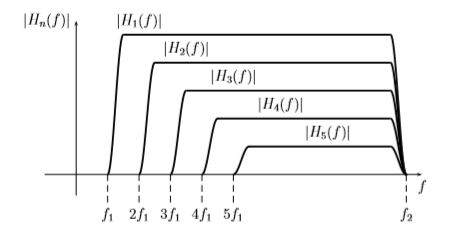
\includegraphics[width=0.6\linewidth]{figuras/NLCFR}
	\caption{Módulo da resposta frequencial dos impulsos. Autor:\cite{novakdissertation}}
	\label{fig:nlcfr}
\end{figure}

Na figura \ref{fig:nlcfr}, as frequências $f_{1}$ e $f_{2}$ são as frequências em que o sinal de excitação começa e termina, respectivamente.

\section{Metodologia utilizada para caracterizar um modelo}\label{Metodologia}

Utilizando o método de caracterização proposto por Farina em \cite{farina2001non} e por Novak em \cite{novak2010nonlinear}, que consiste em alimentar um sistema não linear com um sinal senoidal que varia a sua frequência de forma exponencial, criou-se um modelo de amplificador virtual com as características de um modelo físico.

O amplificador utilizado para a caracterização, mostrado na figura \ref{fig:Black}, é um \textit{Blackstar} HT-5 C, composto por uma válvula 12BH7 no pré amplificador e uma ECC83 na parte de amplificação de potência. Diferente da tentativa de caracterização realizada em trabalhos passados, a caracterização foi feita gravando a saída do pré amplificador, simplificando a quantidade de equipamentos utilizados, evitando ao máximo a captação de ruídos para tenta obter o sinal mais limpo de interferências possíveis.

\begin{figure}
	\centering
	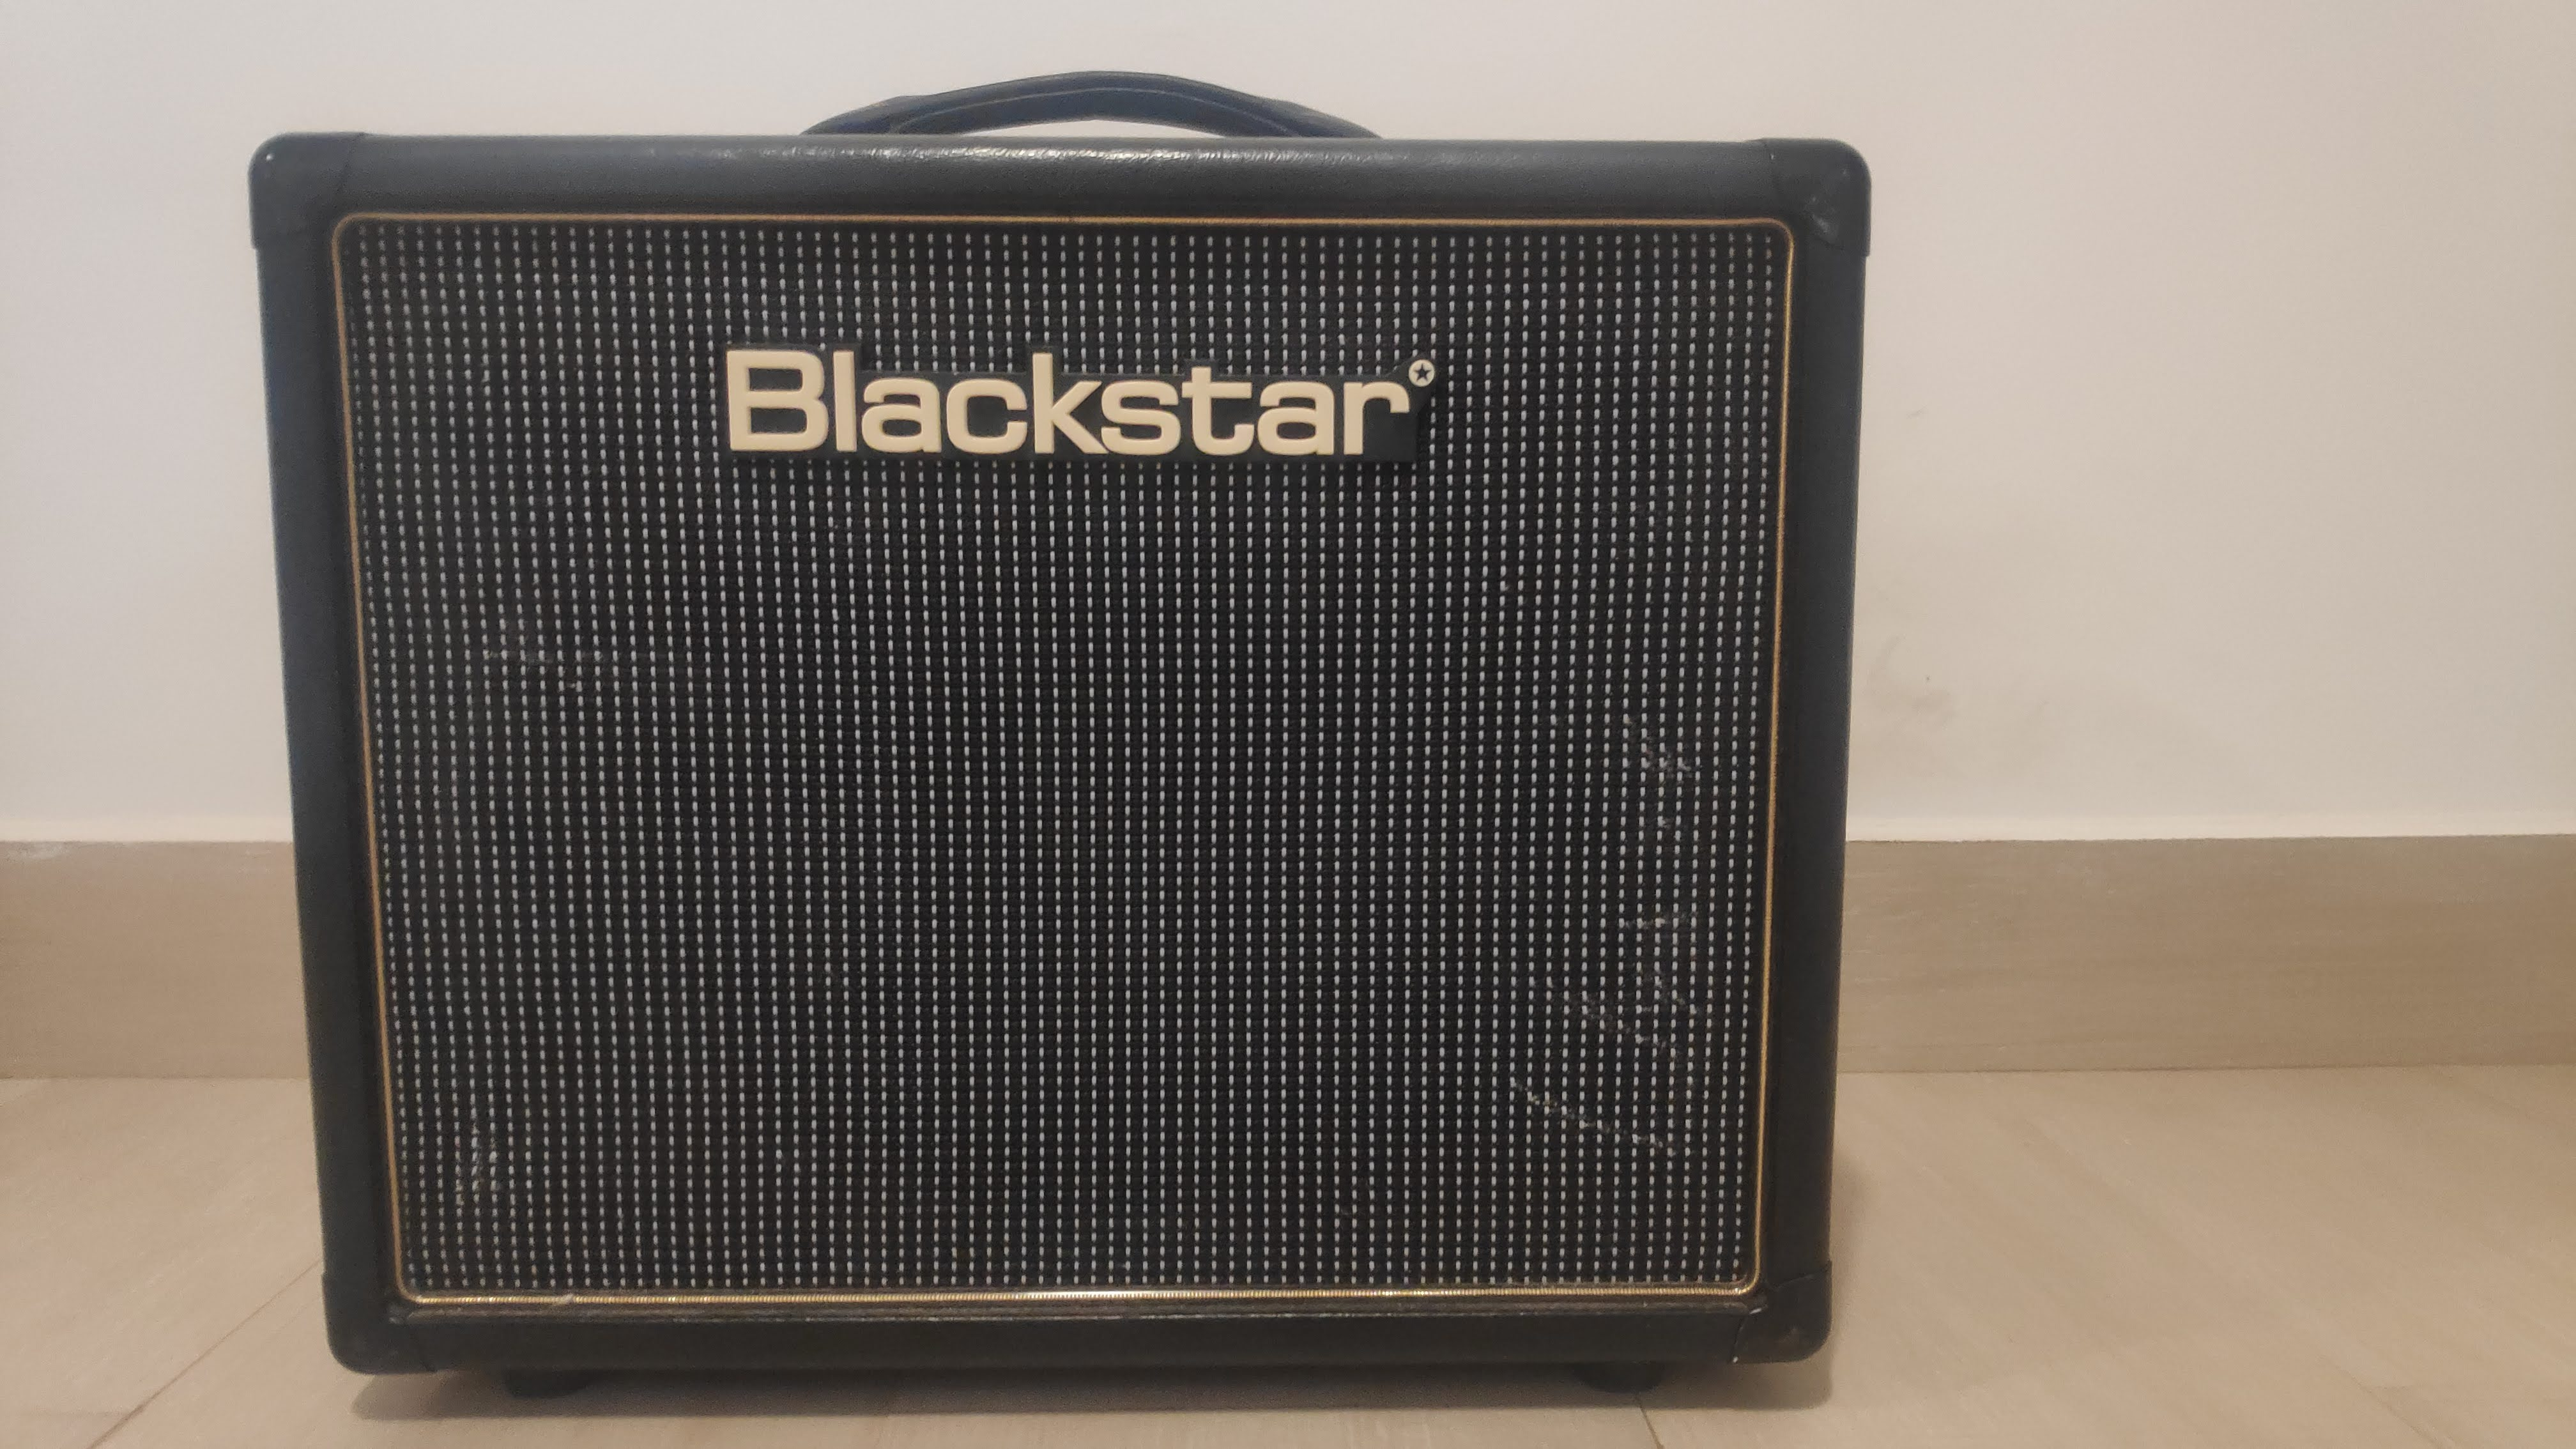
\includegraphics[width=0.5 \linewidth]{figuras/Blackstar1}
	\caption{Amplificador Blackstar HT-5 C}
	\label{fig:Black}
\end{figure}

A criação do sinal de teste foi feita segundo a equação \ref{sinal exponencial}, utilizando o programa Matlab para computar a função e gerar o arquivo de áudio em formato \textit{.wav}. O tempo de duração do sinal foi de 20 segundos, gerando 882000 amostras, devido a frequência de amostragem de 44,1 kHz que foi igualada a frequência da interface de áudio USB utilizada durante o processo de gravação dos sinais.


O sinal exponencial então foi exportado em uma trilha mono, para o programa Audacity, que é um editor, gravador e reprodutor de áudio e configurada para enviar o sinal para a saída da interface. Utilizando a interface de áudio M-audio \textit{Fast Track Pro}, conectou-se a saída do pré amplificador presente no \textit{Blackstar} à entrada de áudio da interface, através de um cabo P10. A saída da interface, por onde o sinal exponencial é enviado do computador, foi conectada à entrada de instrumentos do amplificador. No software Audacity, foi criada uma segunda trilha de áudio armada para gravar o sinal na entrada da interface. 


A figura \ref{fig:diag} mostra como foram feitas as conexões entre computador, interface e amplificador.
\begin{figure}
	\centering
	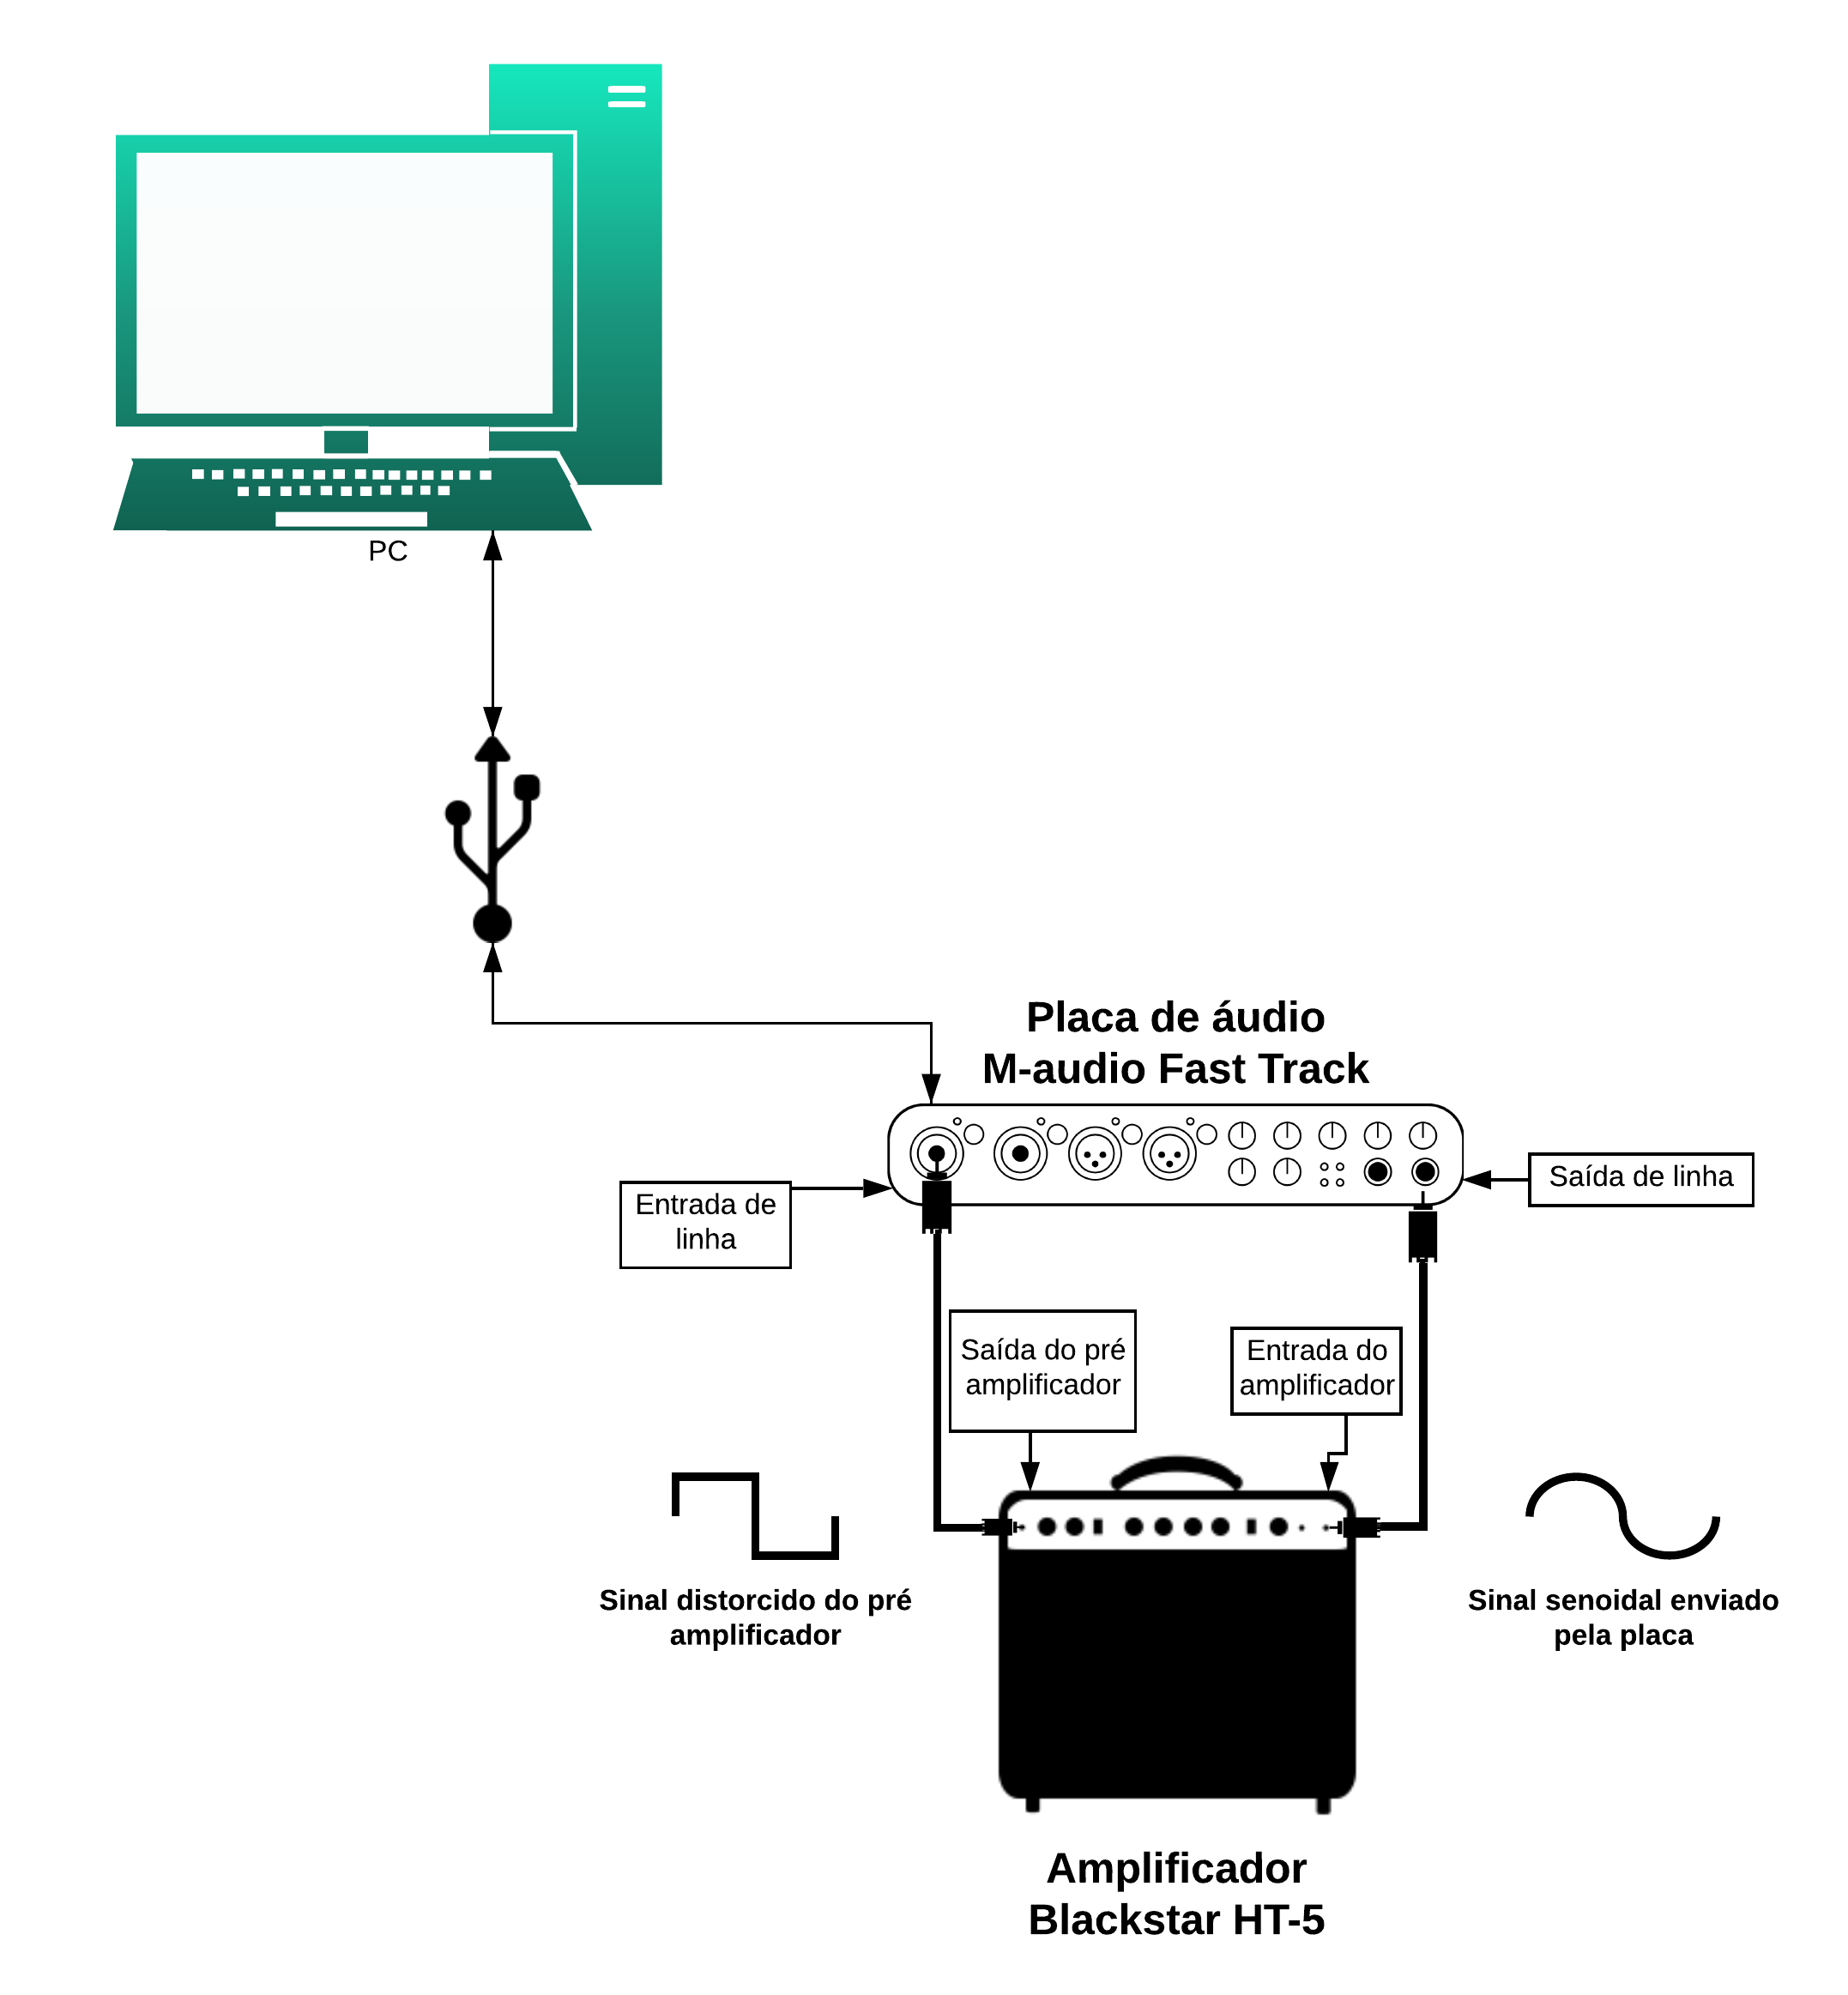
\includegraphics[width=0.7\linewidth]{figuras/diag}
	\caption{Diagrama de conexão do sistema de caracterização}
	\label{fig:diag}
\end{figure}

Após a gravação do sinal exponencial na saída do pré amplificador, o arquivo contendo as informações foi exportado para o Matlab onde foi processado e convoluído com o sinal exponencial invertido para obtenção dos \kernels, como mostra a figura \ref{fig:nlcm}. Seguindo a extração dos \kernels, separou-se cada impulso obtido para a construção do modelo de \textit{Hammerstein} do amplificador, exemplificado na figura \ref{fig:hammer}


\begin{figure}
	\centering
	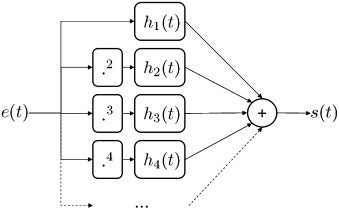
\includegraphics[width=0.5\linewidth]{figuras/hammer}
	\caption{Modelo de \textit{Hammerstein}. Retirado de: https://ars.els-cdn.com/content/image/1-s2.0-S0022460X10006176-gr1.jpg}
	\label{fig:hammer}
\end{figure}

\pagebreak
A ordem do sistema, ou seja, a quantidade de \kernels utilizados para construir o modelo de \textit{Hammerstein}, foi ajustada para utilizar 11 \kernels. A saída do sistema então foi obtida, com a convolução de 11 sinais, cada um elevado a um expoente, cujo valor máximo é determinado pela ordem do sistema, com o \kernels associado a cada expoente. Esses sinais são somados e resultando em um único sinal de áudio que representa a saída final do modelo caracterizado. A figura \ref{fig:diagramamatlab} exemplifica o funcionamento do algorítimo criado para a simulação do amplificador caracterizado.


\begin{figure}[!htb]

	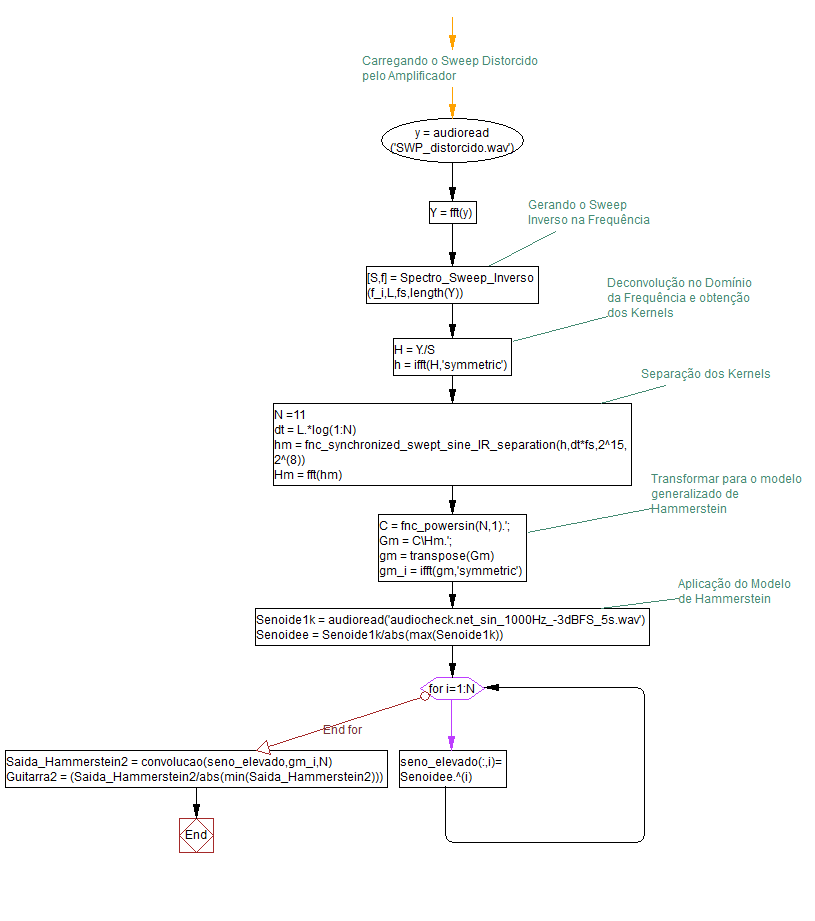
\includegraphics[width=1.0\linewidth]{figuras/Diagrama_Matlab}
	\caption{Fluxograma do programa desenvolvido}
	\label{fig:diagramamatlab}
\end{figure}
